%%%%%%%%%%%%%%%%%%%%%%%%%%%%%%%%%%%%%%%%%%%%%%%%%%%%%%%%%%%%%%%
%
% Arxiu pregenerat.
% NO EDITAR
%
%%%%%%%%%%%%%%%%%%%%%%%%%%%%%%%%%%%%%%%%%%%%%%%%%%%%%%%%%%%%%%%
%doc: SORTIDA MIQUEL BARCELO/barcelo.doc
\begin{news}
{2} %columnes
{Sortida al CaixaForum}
{Miquel Barceló – La Solitude Organisative}
{ESO}
{12} %pagesof

\noindent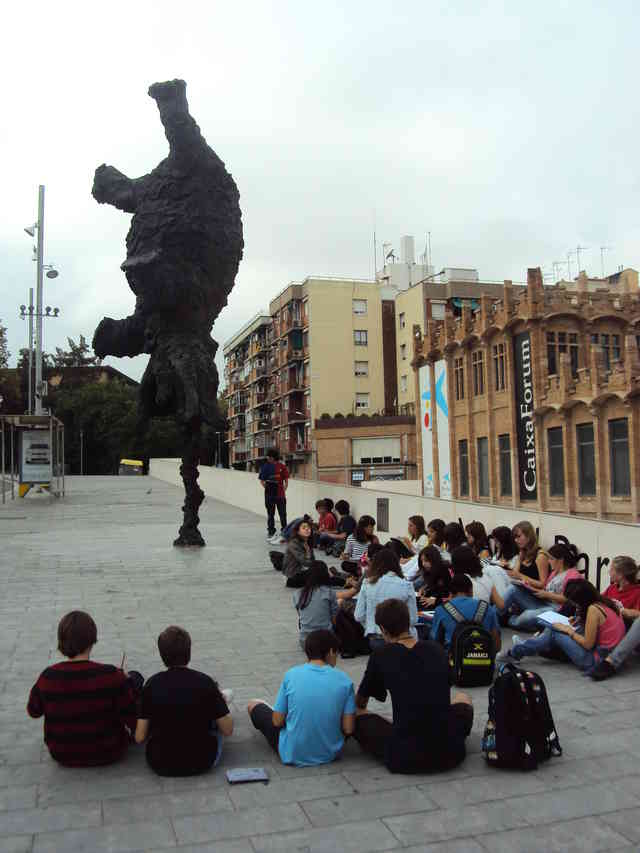
\includegraphics[width=9cm,keepaspectratio]{eso/img/gen/barcelo_dpi_lowres.jpg}


Miquel Barceló.
Miquel Barceló és un pintor mallorquí caracteritzat, entre altres coses, per pintar quadres amb volum, com per exemple el quadre d'una paella, on hi enganxa arròs real. Va estudiar a París, Mali i Mallorca. No creu en Déu, ho demostra amb un quadre en el que canvia la imatge de Jesús crucificat, per un conill crucificat. L’artista també es caracteritza per fer escultures de bronze.

Exposició.
En el primer quadre hi surt ell envoltat de llibres i paisatges en procés d'excitació, cosa que ens vol donar a entendre que li encanten els llibres, els quadres, els paisatges naturals, i que té un gran potencial artístic.

La segona obra és un quadre on hi apareixen diferents animals entre els quals destaca una cabra. En aquesta obra es pot veure una característica de Barceló: dóna volum als seus quadres a l’atzar i, depenent de la forma que adoptin, hi pinta a sobre, improvisant.

Al tercer quadre hi apareix una paella amb arròs real enganxat. També hi apareixen altres aliments com musclos, tomàquets i altres tipus de marisc i d’hortalisses. 

Al quart quadre hi apareixen dues papaies. Aquesta obra es caracteritza perquè la va pintar davant de casa seva, al carrer. El paper del quadre està arrugat perquè la pintura s’escampi per les petites arrugues de la làmina.

L’ obra següent representa un retrat d’un amic seu de l’Àfrica. Es caracteritza perquè ha aprofitat el paper de les papaies per pintar-hi darrere.
 
La sisena obra és una vitrina amb diferents escultures petites fetes amb fang i de diferents formes.

El setè quadre representa la sorra del desert d’Àfrica, pintada d’un blanc trencat, ja que en aquell moment la llum del Sol l’enlluernava.

La vuitena obra és un “collage” de gossos, ja que els compara amb els humans.

A la novena obra hi apareixen diferents quadres de pobles pobres, indígenes, en una paret. Aquest quadre es caracteritza perquè Barceló va deixar el quadre sense pintar al seu estudi i,  quan va tornar, els tèrmits havien fet forats al quadre i ell, en comptes de llençar-lo, va trobar-lo encara més interessant i hi va pintar a sobre, aprofitant els forats.

La desena obra són quadres fets amb elements de la naturalesa (pintures sintètiques, sang d'animals, etc...).

L’onzena obra són diferents quadres en blanc, negre i marró en una sala fosca. Els va pintar a la nit. Amb la foscor vol representar el fons marí, perquè li agradava molt bussejar per les platges de Mallorca.

La darrera obra és una sala de fons vermell amb diferents quadres, uns amb volum i d’altres sense. Hi ha un retrat de la seva biògrafa; també un retrat del seu marxant, i un autoretrat seu. És l’ obra més gran i més destacada de l’ exposició, en la qual es representa a ell mateix com un goril·la, per la seva solitud: d’aquí ve el títol de l’exposició La Solitude Organisative.

\authorandplace{Eduard Ferrusola i Davínia Vilagrasa}{ESO}
\end{news}
